\documentclass[12pt]{article}
\usepackage[T1]{fontenc}
%\usepackage[latin9]{inputenc}
\usepackage[utf8]{inputenc}
\usepackage[english]{babel}
\usepackage{amsmath}
\usepackage{amsfonts}
\usepackage{amssymb}
%\usepackage{setspace}
\usepackage{rotating}
\usepackage{graphics}
\usepackage{eurosym}
\usepackage[round]{natbib}
%\usepackage{graphicx}
%\usepackage{float} 				%allows you to float images
\usepackage{latexsym}
%\usepackage{bbding}
%\usepackage {moresize}
\usepackage{listings}
\usepackage{bbding}
\usepackage{blindtext}
\usepackage{hhline}
\usepackage{tikz}
\usetikzlibrary{trees}
%\usetikzlibrary{shapes,backgrounds}
%\usepackage{pgfplots}
%\usetikzlibrary{arrows}
\usepackage{enumitem}
%\doublespacing
%\usepackage{geometry}
\usepackage{amsthm}
\usepackage{color}
%\usepackage{array,multirow}
%\usepackage{subcaption}
%\usepackage{pst-plot}
%	\psset{xunit=15mm}
%\geometry{verbose,tmargin=1in,bmargin=1in,lmargin=.5in,rmargin=.5in}
\setlength{\parskip}{\bigskipamount}
\setlength{\parindent}{0pt}
\usepackage{multicol}

\newenvironment{problem}[3][Problem]{\begin{trivlist}
\item[\hskip \labelsep {\bfseries #1}\hskip \labelsep {\bfseries #2.}]}{\end{trivlist}}

\newcommand{\barr}{\bar{r}}
\newcommand{\ddx}{\frac{d}{dx}}
\newcommand{\infsum}{\sum_{n=1}^{\infty }}

\title{Problem Set 5 \thanks{Problems:5.2,5.4,5.6,5.7,5.12,5.16,5.17,5.20,5.27}}
\author{Ian McGroarty \\
	Course Number: 555.444}
\date{September 30, 2019}

\begin{document}

\maketitle
\newpage
%%%%%%%%%%%%%%%%%%%%%%%%%%%%%%%%%%%%%%%%%%%%%%%%%%%%%%%%
%%%%%%%%%%%%%%%%%%%%%%%%%%%%%%%%%%%%%%%%%%%%%%%%%%%%%%%%
%%%%%%%%%%%%%%%%%%%%%%%%%%%%%%%%%%%%%%%%%%%%%%%%%%%%%%%%
\begin{problem}{6.4}. A Eurodollar futures price changes from 96.76 to 96.82. What is the gain/loss for an investor who is long two contracts. 

Okay so, they are long Eurodollar futures contracts. Which means they will purchase them later. The settlement is 100-R, so a higher R (closer to 100 \#looking at you Germany)  means that you have to pay less.  So if the price (R) rises, they benefit. The Eurodollar contract is designed so that a one-basis point move in the futures quote corresponds to a gain of \$25 per contract. So the final settlement on the contract is: $$ 2 * 25*(9682-9676) = \$300 $$
\end{problem}

\begin{problem}{6.6}. The 350-day LIBOR rate is 3\% with continuous compounding and the forward rate calculated from a Eurodollar futures contract that matures in 350 days is 3.2\% with continuous compounding. Estimate the 440-day zero rate. 

I\rq{}m going to assume that \lq\lq{}matures in 350 days\rq\rq{} means begins in 350 days. But I\rq{}m unclear as to why? 
\begin{align*}
F_i &= \frac{R_{i+1}T_{i+1}-R_iT_i}{T_{i+1}-T_i} && \text{Eqn. 6.4 (og. 147)}\\
&= \frac{0.032*90 + 0.03*350}{440} \\
&= 0.03040909
\end{align*}
\end{problem}

\begin{problem}{6.9}. It is May 5, 2014. The quoted price of a government bond with a 12\% coupon that matures on July 27, 2024, is 110-17. What is the cash price? 

I\rq{}ll assume that government bond is a Treasury bond not a municipal bond which would technically also be a Government bond (right?). That means we will use actual/actual day count. We can assume that the last coupon payment is 6 months before July 27, 2014 which is January 27, 2014. There are ... 98 days between 27JAN14-5MAY14 (according to timeanddate.com). There are 181 days between 27JAN14-27JULY14. The accrued interest is thus: $\frac{98}{181} \cdot 0.06 =   0.0324$ Or \$3.24 per \$100 face value of the bond. We can add this to the Quoted price: 
$$110 \frac{17}{32} = 110.531 \implies 110.531 + 3.24 = \$113.78  \text{ cash price of a \$100 bond. }$$
\end{problem}


\begin{problem}{6.11}. It is July 30, 2015. The cheapest-to-deliver bond in a September 2015 Treasury bond futures
contract is a 13\% coupon bond, and delivery is expected to be made on September 30, 2015.
Coupon payments on the bond are made on February 4 and August 4 each year. The term
structure is flat, and the rate of interest with semiannual compounding is 12\% per annum.
The conversion factor for the bond is 1.5. The current quoted bond price is \$110. Calculate
the quoted futures price for the contract

First, there are 62 days until delivery date, 176 days since the last coupon payment, 5 days until the next coupon payment. 
We can thus calculate the cash price using the actual/actual method since it is a treasury bond: 
$$ 110 + \frac{176}{176+5} \cdot \frac{13}{2}  = 116.32$$
Now we need the income received over the period. We can calculate the present value of the next coupon payment of \$6.5 which is in 5 days (= 0.0137 years) using the rate of interest of \%12 per annum: 
$$ 6.5e^{-0.12\cdot 0.0137} = 6.489 $$
So we have the cash value of the bond, the Income. We need to calculate the value at delivery in 62 days (=0.1699 years):
\begin{align*}
F_0 &= (S_0 - I)e^{rT}  && \text{ Eqn. 6.1 (pg. 141)} \\
&= (116.32 - 6.489)e^{0.12\cdot 0.1699} \\
F_0 &= 112.0932
\end{align*}
Now need to subtract the interest accrued in the 57 days between 4AUG15 and 30SEPT15 for the 4FEB16 coupon payment (127 days away) that is never actually received  but makes it\rq{}s way into the calculation above: 
$$ 112.0932 - 6.5 \cdot \frac{57}{127+57} = 110.0796 $$
Finally, we divide this by the conversion factor: $110.0796/1.5 = 73.3864$ which is the quoted futures price.
\end{problem}

\newpage
\begin{problem}{6.14}. REVISIT YOU MAY NEED TO CHANGE THE COMPOUNDING %%%%

Suppose that the 300-day LIBOR zero rate is 4\% and Eurodollar quotes for contracts
maturing in 300, 398 and 489 days are 95.83, 95.62, and 95.48. Calculate 398-day and 489-
day LIBOR zero rates. Assume no difference between forward and futures rates for the
purposes of your calculations:

First note that the EuroDollar quotes are expressed as 100-R, so in order to get the forward rate we must subtract from 100. Then it becomes a straightforward application of( Eqn. 6.4 pg. 147): $R_{i+1} = \frac{F_i(T_{i+1}-T_i) + R_iT_i}{T_{i+1}-T_i} $ See the table below for results:\\
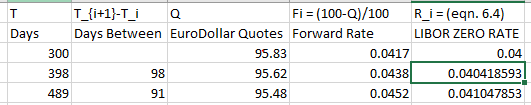
\includegraphics[width=\textwidth]{mod5_p614.png}
\end{problem}



%%%DO THE R FOR THIS 
\begin{problem}{6.21}. The three-month Eurodollar futures price for a contract maturing in six years is quoted as
95.20. The standard deviation of the change in the short-term interest rate in one year is
1.1\%. Estimate the forward LIBOR interest rate for the period between 6.00 and 6.25 years
in the future. 

Well, we see that the futures rate is 100-95.20=4.8\% per annum on an actual/360 basis with quarterly compounding.  We need to translate this into continuous compounding on an annual base:
\begin{align*}
R_c &= m \cdot ln(1+\frac{R_m}{m} && \text{Eqn. 4.3 (pg. 83)} \\
&= 4 \cdot ln(1+\frac{0.048}{4}) \\
R_c &= 0.04771428  && \text{Cont. Comp. Actual/360} \\
Actual/Actual &= 0.04771428 \cdot \frac{365}{360} = 4.838 \\
\text{Forward Rate} &= \text{Futures Rate } - \frac{1}{2}\sigma^2T_1T_2  && \text{Eqn. 6.3 (pg. 146)} \\
&= 4.838 - (\frac{1}{2} \cdot 0.011^2 \cdot 6 \cdot 6.25 \cdot 100)\\ 
\text{Forward Rate} &=  4.611
\end{align*}
\end{problem}


\newpage
\begin{problem}{6.27}. It is 10MAR14 The cheapest-to-deliver Treasury bond futures contract is an 8\% coupon bond, and delivery is expected to be made on 31DEC14. Coupon payments on the bond are made on 1MAR and 1SEPT each year.
The rate of interest with continuous compounding is 5\% per annum for all maturities. The
conversion factor for the bond is 1.2191. The current quoted bond price is \$137. Calculate
the quoted futures price for the contract. 

I\rq{}ve already walked through how to do this, so I\rq{}ll be a bit quicker: Days between; 1MAR14 - 10MAR14 = 9, 1MAR14-1SEPT14 = 184, 10MAR14-1SEPT14 = 175 days = 0.479 years 1SEPT14-31DEC14 = 121 Days, 10MAR14-31DEC14 = 296 Days = 0.811years,  1SEPT14-1MAR15 = 181. 
\begin{align*}
S_0 &= \text{current quote + proportional coupon} \\ 
S_0 &= 137 + \frac{8}{2} \cdot \frac{9}{184} = 137.1957 \\
I &= \frac{8}{2} \cdot e^{-0.05 \cdot 0.479} \\
I &= 3.905 \\
F_0 &= (S_0 - I)e^{rT}  && \text{ Eqn. 6.1 (pg. 141)} \\
F_0&= (  137.1957  -  3.905) \cdot e^{0.05 \cdot 0.811} \\ 
F_0 &= 138.8067\\ 
P_{Deliver} &= F_0 - \text{accrued interest} \\ 
&= 138.8067 - (\frac{8}{2} \cdot \frac{121}{181}) \\
&= 136.1327 \\ 
\text{Quoted Futures Price} &= \frac{P_{Deliver}}{Conversion Factor} \\
\text{Quoted Futures Price}  &= \frac{136.1327 }{1.2191} \\
\text{Quoted Futures Price} & = 111.68
\end{align*}
\end{problem}


\newpage 
\begin{problem}{6.28}. Assume that a bank can borrow or lend money at the same interest rate in the LIBOR market.
The 90-day rate is 10\% per annum, and the 180-day rate is 10.2\% per annum, both expressed
with continuous compounding. The Eurodollar futures price for a contract maturing in 91
days is quoted as 89.5. What arbitrage opportunities are open to the bank? 

First, we have to compare apples to apples. The Eurodollar futres price is quoted at 89.5 meaning the futures rate is 10.5 per annum  on an actual/360 basis with quarterly compounding. 
\begin{align*}
R_c &= m \cdot ln(1+\frac{R_m}{m} && \text{Eqn. 4.3 (pg. 83)} \\
&= 4 \cdot ln(1 + \frac{0.105}{4} \\ 
R_c &= 0.1036  && \text{Cont. Comp. Actual/360} \\
0.1036 \cdot \frac{365}{360} = 0.1051 
\end{align*}
This is the actual/actual day count with continuous compounding. Next, the we calculate the forward rate for the 90 and 180 day:
\begin{align*}
F_i &= \frac{R_{i+1}T_{i+1} - R_iT_i}{T_{i+1}-T_i} \\
&= \frac{10.2*180 - 10*90}{180-90}\\
F_i &= 10.4
\end{align*}
So the Forward rate 10.4\% is less than the Eurodollar futures rate 10.51\%. That means that we could get more from the Eurodollar futures than the forward rate. So we want to borrow money at the forward rate and use that money to buy Eurodollar futures now. You\rq{}ll need to reevaluate in 90 days when the EuroDollar future matures. 
\end{problem}

\newpage
\begin{problem}{6.29}. A Canadian company wishes to create a Canadian LIBOR futures contract from a U.S.
Eurodollar futures contract and forward contracts on foreign exchange. Using an example,
explain how the company should proceed. For the purposes of this problem, assume that a
futures contract is the same as a forward contract. 


I\rq{}ll admit that I am a little confused by this one. So we want to lock in a exchange rate between the canadian interest rate and the libor rate using Eurodollar futures. But I take it this means EuroUSD not EuroCAD because otherwise you\rq{}d just get EuroCanadianDollar futures. If this is the case then what you\rq{}d have to do it buy USD now, and take a long contract to purchase CAD (with USD) 3 months from now. Thus, you have fixed the exchange rate. Use the USD to purchase Eurodollar futures thereby locking in the interest rate. In 3 months, you\rq{}ll get your USD + Eurodollar interest. Use that money to buy back the CAD and you\rq{}re all set. 
\end{problem}
\end{document}



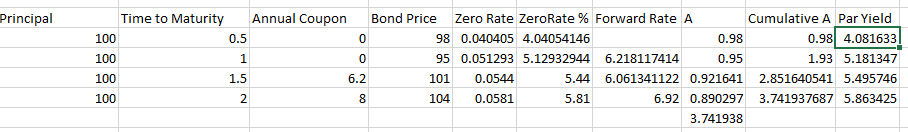
\includegraphics[width=\textwidth]{mod3_p434.png}
% Set the overall layout of the tree




\tikzstyle{level 1}=[level distance=3.5cm, sibling distance=3.5cm]
\tikzstyle{level 2}=[level distance=3.5cm, sibling distance=2cm]

% Define styles for bags and leafs
\tikzstyle{bag} = [text width=4em, text centered]
\tikzstyle{end} = [circle, minimum width=3pt,fill, inner sep=0pt]

\begin{tikzpicture}[grow=right, sloped]
\node[bag] {Bag 1 $4W, 3B$}
    child {
        node[bag] {Bag 2 $4W, 5B$}        
            child {
                node[end, label=right:
                    {$P(W_1\cap W_2)=\frac{4}{7}\cdot\frac{4}{9}$}] {}
                edge from parent
                node[above] {$W$}
                node[below]  {$\frac{4}{9}$}
            }
            child {
                node[end, label=right:
                    {$P(W_1\cap B_2)=\frac{4}{7}\cdot\frac{5}{9}$}] {}
                edge from parent
                node[above] {$B$}
                node[below]  {$\frac{5}{9}$}
            }
            edge from parent 
            node[above] {$W$}
            node[below]  {$\frac{4}{7}$}
    }
    child {
        node[bag] {Bag 2 $3W, 6B$}        
        child {
                node[end, label=right:
                    {$P(B_1\cap W_2)=\frac{3}{7}\cdot\frac{3}{9}$}] {}
                edge from parent
                node[above] {$B$}
                node[below]  {$\frac{3}{9}$}
            }
            child {
                node[end, label=right:
                    {$P(B_1\cap B_2)=\frac{3}{7}\cdot\frac{6}{9}$}] {}
                edge from parent
                node[above] {$W$}
                node[below]  {$\frac{6}{9}$}
            }
        edge from parent         
            node[above] {$B$}
            node[below]  {$\frac{3}{7}$}
    };
\end{tikzpicture}


\section{Definitions}
\underline{Def: Forward Rate Formulas} (pg 79). The implied forward rate between times $t_1$ and $t_2$ is the rate of interset between those times that is consistent with a given spot rate curve. For Yearly compounding, the forward rate is:  
\begin{align*}
f_{i,j} =& [\frac{(1+s_j)^j}{(1+s_i)^i}]^{1/(j-i)}-1 \\
 e^{s(t_2)t_2} =& e^{s(t_1)t_1}e^{f_{t_1,t_2}(t_2-t_1)}
\end{align*}

\underline{Discount Factor Relation} The discount facot between periods i and j is defined as $$ d_{i,j}=[\frac{1}{1+f_{i,j}}]^{j-i}$$ These factors satisfy the compounding rule: $d_{i,k}=d_{i,j}d_{j,k}$\\

\underline{Def. Derivative (Ross pg 223)} Let F be a real valued function defined on an open interval contained a point a. We say f is differentiable at a, or f has derivative at a if the limit $$ f'(a) = \lim_{x \to a} \frac{f(x)-f(a)}{x-a} $$




https://www.investopedia.com/university/advancedbond/bond-pricing.asp
https://quant.stackexchange.com/questions/22288/duration-of-perpetual-bond
http://people.stern.nyu.edu/gyang/foundations/sample-final-solutions.html
http://pages.stern.nyu.edu/~jcarpen0/courses/b403333/07convexh.pdf
https://web.stanford.edu/class/msande247s/2009/summer%2009%20week%205/Bond%20Formula%20Sheet.pdf


\underline{Def: Forward Rate Formulas} (pg 79). The implied forward rate between times $t_1$ and $t_2$ is the rate of interset between those times that is consistent with a given spot rate curve. For Yearly compounding, the forward rate is:  
\begin{align*}
f_{i,j} =& [\frac{(1+s_j)^j}{(1+s_i)^i}]^{1/(j-i)}-1 \\
 e^{s(t_2)t_2} =& e^{s(t_1)t_1}e^{f_{t_1,t_2}(t_2-t_1)}
\end{align*}

\underline{Discount Factor Relation} The discount facot between periods i and j is defined as $$ d_{i,j}=[\frac{1}{1+f_{i,j}}]^{j-i}$$ These factors satisfy the compounding rule: $d_{i,k}=d_{i,j}d_{j,k}$\\

\underline{Def. Derivative (Ross pg 223)} Let F be a real valued function defined on an open interval contained a point a. We say f is differentiable at a, or f has derivative at a if the limit $$ f'(a) = \lim_{x \to a} \frac{f(x)-f(a)}{x-a} $$



\begin{align*}
\text{Maximize  } & 4x_1 +5x_2 +3x_3 +4.3x_4 + x_5 + 1.5x_6 + 2.5x_7 + 0.3x_8 + x_9 + 2x_{10} \\
\text{Subject to } & 2x_1 + 3x_2 + 1.5x_3 + 2.2x_4 +0.5x_5 +15x_6 + 2.5x_7 +0.1x_8 + 0.6x_9 + x_{10} \leq 5 \\ 
& x_1 + x_2 + x_3 + x_4 \leq 1 \\
& x_5 + x_6 + x_7 \leq 1 \\
& x_8 + x_9 + x_{10} \leq 1 \\
\end{align*}